%TCIDATA{Version=5.00.0.2606}
%TCIDATA{LaTeXparent=0,0,..\Elvira-Book.tex}

%TCIDATA{ChildDefaults=chapter:1,page:1}


\section{Influence diagrams in Elvira GUI}

The Elvira Graphical User Interface (Elvira GUI) is a complete environment
to develop systems based in probabilistic graphical models. In this section
we are going to explain its capabilities related with IDs, as edition,
evaluation or reasoning explanation. However, given the dynamic development
and implementation of algorithms in Elvira system, the GUI only cover a part
of all capabilities that Elvira has got related with IDs. Then, we will see
through a trip across the Elvira GUI all this program offers to the user
about IDs.

The trip starts seeing how an ID is presented in the Elvira GUI. Let us
consider the ID of a known problem of decision making: the oil wildcatter
problem. In Figure \ref{fig:reactorIDGUI} the ID is displayed in the edition
environment of Elvira GUI. The acyclic directed graph of the ID is
displayed, where we can appreciate the three kinds of nodes: decision
(graphically represented by squares or rectangles), chance (circles or
ovals) and utilities (diamonds).

\begin{figure}[h]
\begin{center}
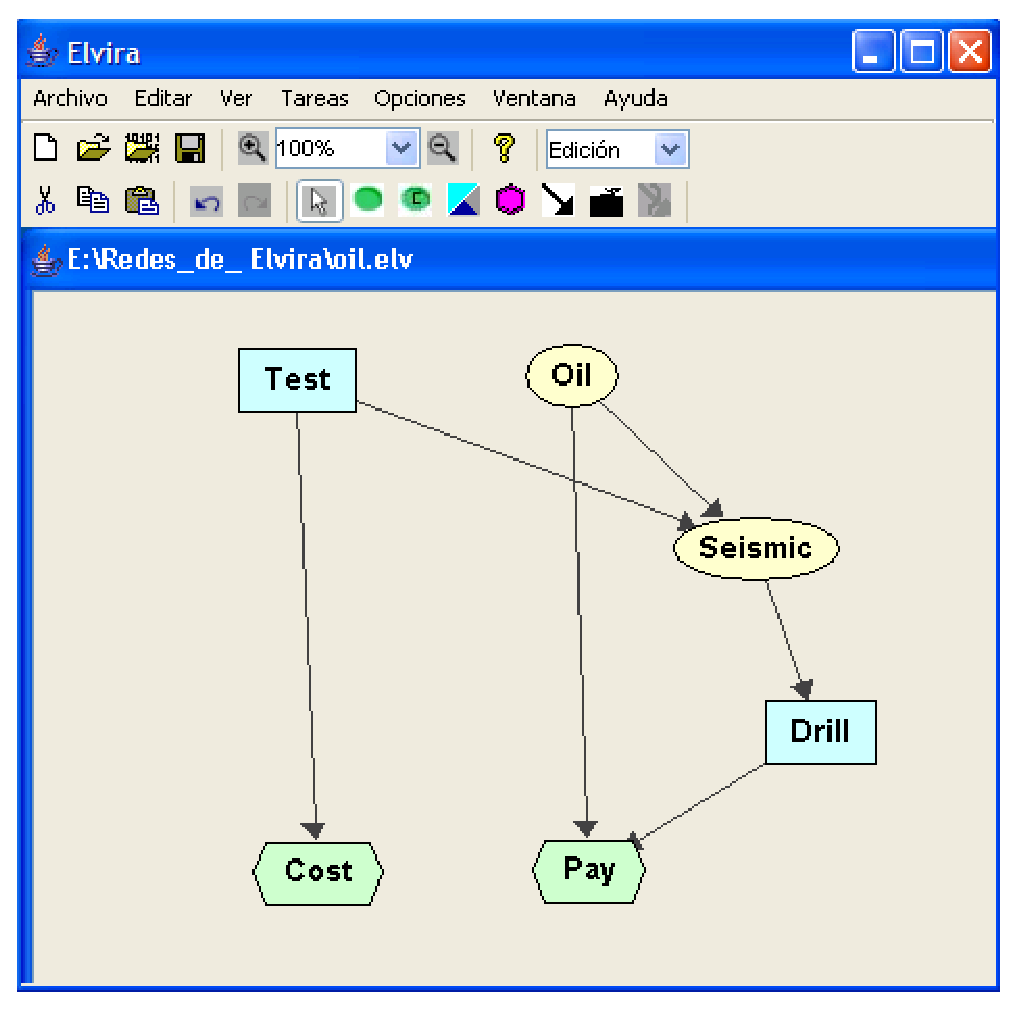
\includegraphics[scale=0.6]{./ID/fig/reactorIDGUI} \vspace{-0.5cm}
\end{center}
\caption{An ID in the edition environment of Elvira GUI}
\label{fig:reactorIDGUI}
\end{figure}

Now, we are going to describe how IDs as of the Figure \ref{fig:reactorIDGUI}
can be edited and evaluated. So, we will see how the edition and evaluated
of IDs are performed through two modes which determine the functionality of
the Elvira GUI: \textit{Edition }and \textit{Inference.} The mode is
indicated in the toolbar of Elvira. For example, the Spanish word \textit{%
"Edici\'{o}n"} in the toolbar of Figure \ref{fig:reactorIDGUI} indicate us
that the Elvira GUI is in mode \textit{Edition.}

\subsection{Edition of influence diagrams in Elvira GUI}

The edition of an IDs is very similar to the edition Bayesian networks. Let
us suppose we want to create the ID of Figure \ref{fig:reactorIDGUI}. First,
we draw the graph of the ID. We could follow the next steps.

\begin{enumerate}
\item In order to create the ID, we click on \textit{File }and\textit{\ New
network }of the main menu of Elvira, select \textit{Influence Diagram} and
write a title for our example.

\item We introduce the nodes of the ID by selecting the icon corresponding
in the toolbar of Elvira and dragging it to the desired place of the Elvira
pane. The icon of a chance node is an oval, while squares and diamonds are
the icons of decision and utility nodes respectively.

\item We introduce the arcs of the graph by selecting the arrow situated on
the toolbar and tracing the arc from the origin node to the destiny node.
\end{enumerate}

Now, we have to introduce the quantitative information of the ID, i.e., the
probabilities and the utilities. Elvira can set some of this quantitative by
default during the edition of the ID. However, it is likely that we want to
change it. The steps that we have to follow are explained.

\begin{enumerate}
\item If we double-click a chance node Elvira displays its probability
distribution associated. For example, Figure \ref{fig:editProb} shows the
probability distribution $p(Seismic|Oil,Test)$ associated to the node $%
Seismic.$ This table could be edited by changing the numerical values or the
kind of probability distribution (general, numerical trees, canonical
models, etc.).

\item We can edit the utilities of an utility node by double-clicking it
(see utilities of node $Pay$ in Figure \ref{fig:editUtil}).

\item Elvira assumes that there exists a sum among the utility nodes when
they do not have any children. This is the case for the oil wildcatter
problem (Figure \ref{fig:reactorIDGUI}). However, Elvira GUI let us have
super-value nodes. So, we can by double-click a super-value node, drag it
into Elvira pane and mark if the super-value node is a sum or a product. For
example, in spite of the fact that it is not required for the oil wildcatter
problem, we would be able to add a sum node to the ID and obtain the ID with
super-value nodes of Figure \ref{fig:reactorIDSVGUI}.
\end{enumerate}

\begin{figure}[h]
\begin{center}
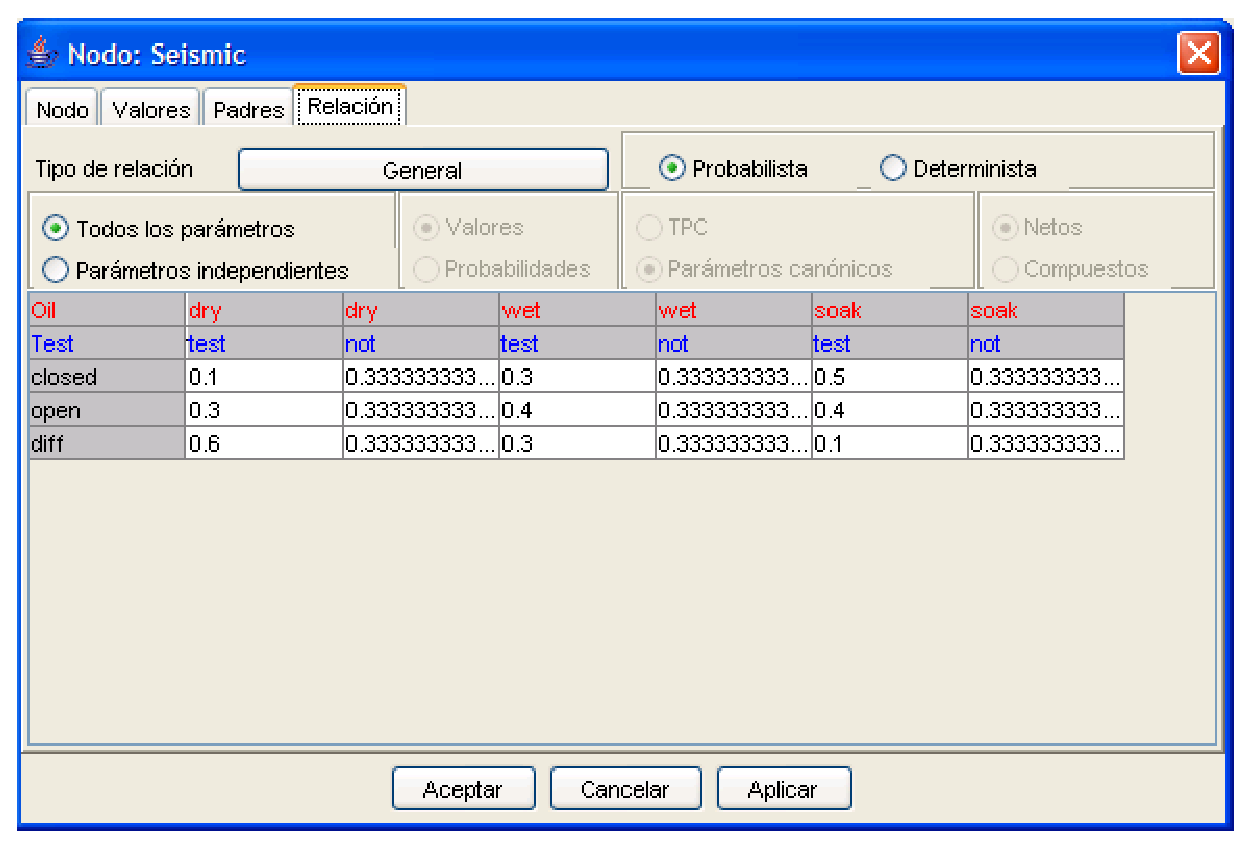
\includegraphics[scale=0.3]{./ID/fig/editProb.eps} \vspace{-0.5cm}
\end{center}
\caption{Probability distribution of a chance node}
\label{fig:editProb}
\end{figure}

\begin{figure}[h]
\begin{center}
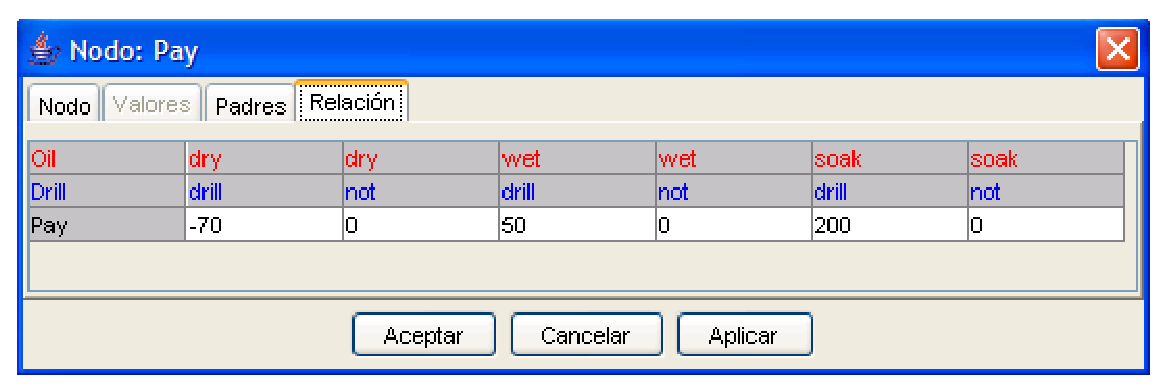
\includegraphics[scale=0.35]{./ID/fig/editUtil.eps} \vspace{-0.5cm}
\end{center}
\caption{Utilities associated to the node \textit{Pay}}
\label{fig:editUtil}
\end{figure}

\begin{figure}[h]
\begin{center}
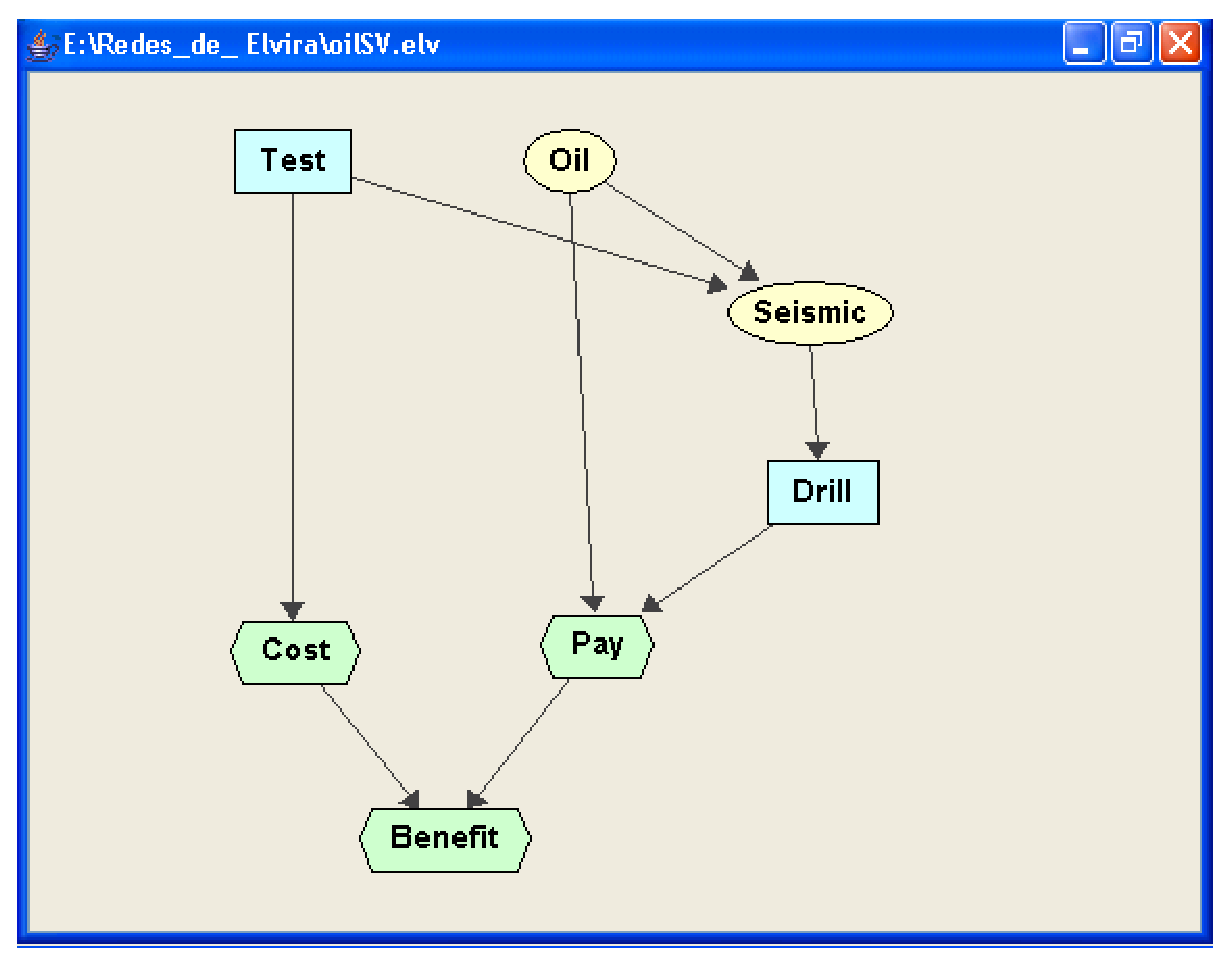
\includegraphics[scale=0.35]{./ID/fig/reactorIDSVGUI.eps} \vspace{-0.5cm}
\end{center}
\caption{An ID with super-value nodes equivalent to Figure \protect\ref%
{fig:reactorIDGUI}}
\label{fig:reactorIDSVGUI}
\end{figure}

\subsection{Evaluation of influence diagrams in Elvira GUI}

The first step to evaluate an ID is to select the propagation method. If we
click on \textit{Options} and \textit{Propagation Method} we can choose
among four groups of algorithms. Figure \ref{fig:selectAR} displays the
selection of the evaluation method. Next, we present these groups of
algorithms.

\begin{itemize}
\item \texttt{Arc reversal. }It evaluates the ID with the arc-reversal
algorithm. It has got three variants that let us evaluate by using
potentials trees and constraints.

\item \texttt{Variable elimination. }The ID is evaluated by applying the
variable elimination algorithm. As in the case of arc-reversal, we can use
three variants of the algorithm that include potential trees and constraints.

\item \texttt{Tatman and Shachter. }The evaluation of the ID is performed
according to Tatman and Shachter's algorithm. Although the optimal policies
are always calculated with this algorithm, we can decide if it has to
compute the utilities of the policies.

\item \texttt{Variable elimination for IDs with super-value nodes. }The ID
is evaluated with the algorithm variable elimination for IDs with
super-value nodes. There are two variants of this algorithm: with or without
divisions. As in Tatman and Shachter's algorithm, if we choose performing
divisions we can decide if it has to compute the utilities of the policies.
\end{itemize}

\begin{figure}[h]
\begin{center}
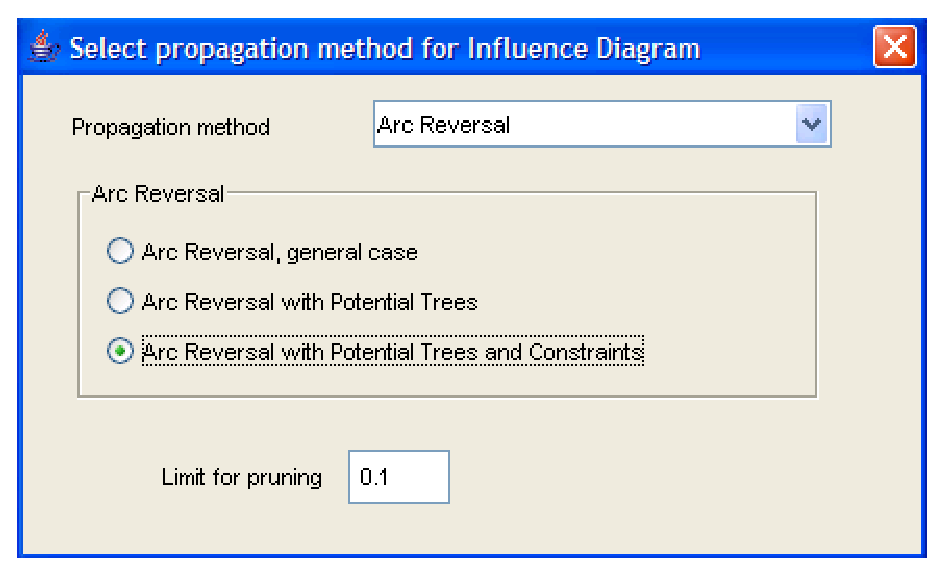
\includegraphics[scale=0.4]{./ID/fig/selectAR.eps} \vspace{-0.5cm}
\end{center}
\caption{Selecting the arc-reversal algorithm}
\label{fig:selectAR}
\end{figure}

When we change the mode of Elvira from \textit{Edition }to \textit{Inference
}mode the ID is evaluated. The aspect that Elvira presents when the ID of
Figure \ref{fig:reactorIDSVGUI} can be seen in Figure \ref%
{fig:evaluatedReactorIDSVGUI}, showing very interesting information for the
decision maker.

\begin{figure}[h]
\begin{center}
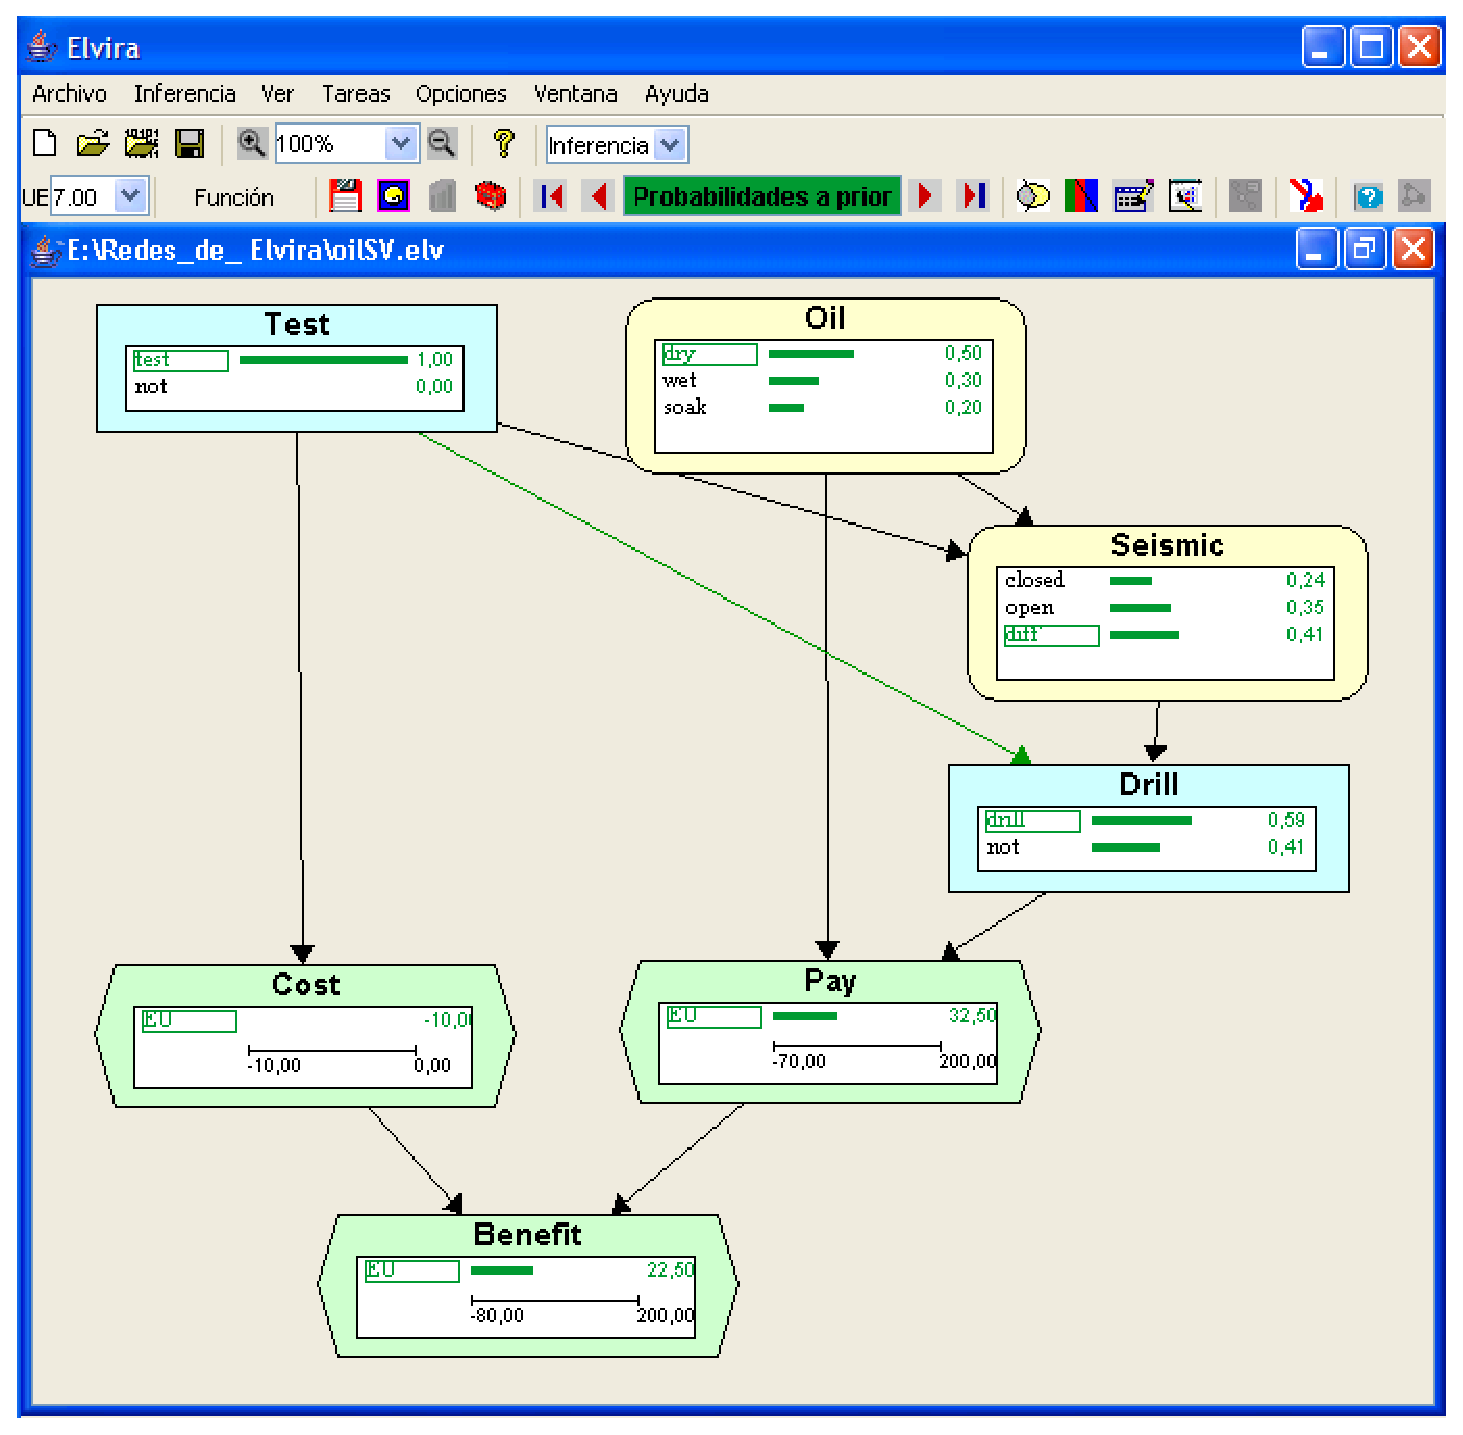
\includegraphics[scale=0.35]{./ID/fig/evaluatedReactorIDSVGUI.eps} \vspace{-0.5cm}
\end{center}
\caption{Evaluated ID in the \textit{Inference} mode}
\label{fig:evaluatedReactorIDSVGUI}
\end{figure}


First, Elvira exhibits the maximum expected utility for the complete
decision problem. That value is shown in the node $Benefit$ of Figure \ref%
{fig:reactorIDSVGUI}, which is a super-value node without successors that
represents the global utility of the problem. Partial utilities can also be
known in non-terminal utility nodes like $Cost$ or $Pay$. This can be
appreciated more clearly in Figure \ref{fig:utilityExpanded}, where a guide
bar indicates the maximum and minimum values of the utility function of the
node $Pay,$ while an horizontal bar indicates the expected utility for that
node.

\begin{figure}[h]
\begin{center}
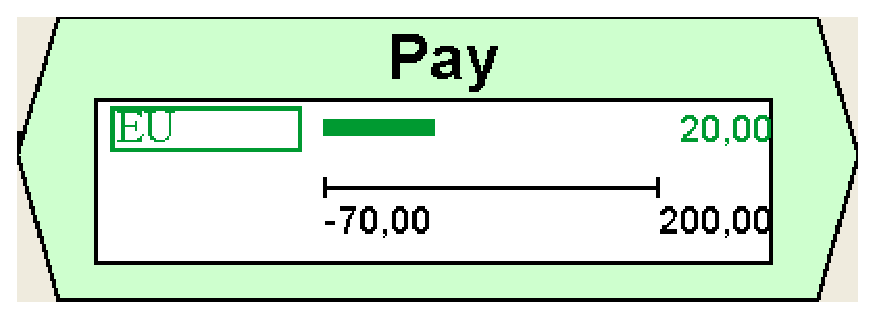
\includegraphics[scale=0.4]{./ID/fig/utilityExpanded.eps} \vspace{-0.5cm}
\end{center}
\caption{Expected utility for a utility node}
\label{fig:utilityExpanded}
\end{figure}

Other interesting information offered by Elvira consists in the
probabilities and utilities of each decision scenario. For example, Figure %
\ref{fig:distribPosteriori} displays the posterior probability distribution
of node $Oil$. Also, we can see in Figure \ref{fig:utilPosteriori} the
utility of each decision scenario, i.e., the expected utility of each state
of the variable.

\begin{figure}[h]
\begin{center}
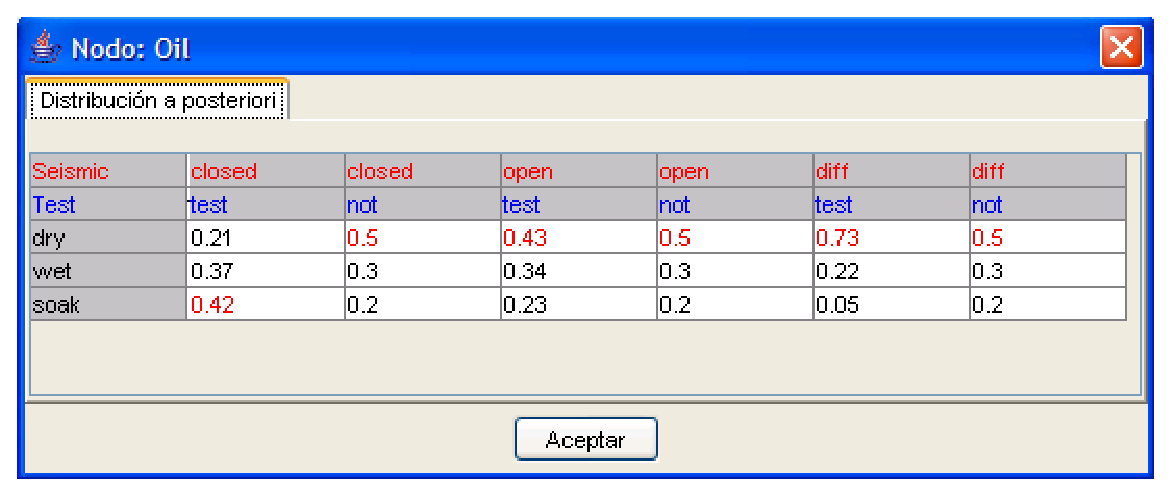
\includegraphics[scale=0.4]{./ID/fig/distribPosteriori.eps} \vspace{-0.5cm}
\end{center}
\caption{Probabilities of the scenarios for $Oil$}
\label{fig:distribPosteriori}
\end{figure}

\begin{figure}[h]
\begin{center}
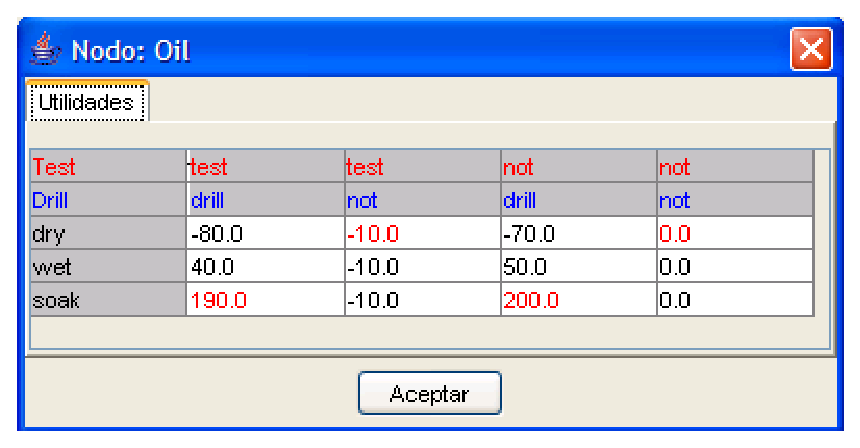
\includegraphics[scale=0.4]{./ID/fig/utilPosteriori.eps} \vspace{-0.5cm}
\end{center}
\caption{Utilities of the scenarios for $Oil$}
\label{fig:utilPosteriori}
\end{figure}

The decision maker can also examine the optimal policy when the
values of certain variables are known. This can be very useful in
some applications like medical decision problems, where it let us
study a subpopulation of the patients instead of the general
population. For example, if we know that the result of the test
$Seismic$ was $closed$, Figure \ref{fig:evaluatedCaseReactorIDSVGUI}
reveals which would be the new probabilities for the states of the
variable $Oil$, and how the optimal decision of $Drill$ would be
$drill$. Furthermore, the new values are compared graphically with
the values obtained when we have not any previous information (the
horizontal bars are duplicated in each state and drawn with a
different color for each situation). Finally, utility nodes exhibit
the expected utilities for the new case.

\begin{figure}[h]
\begin{center}
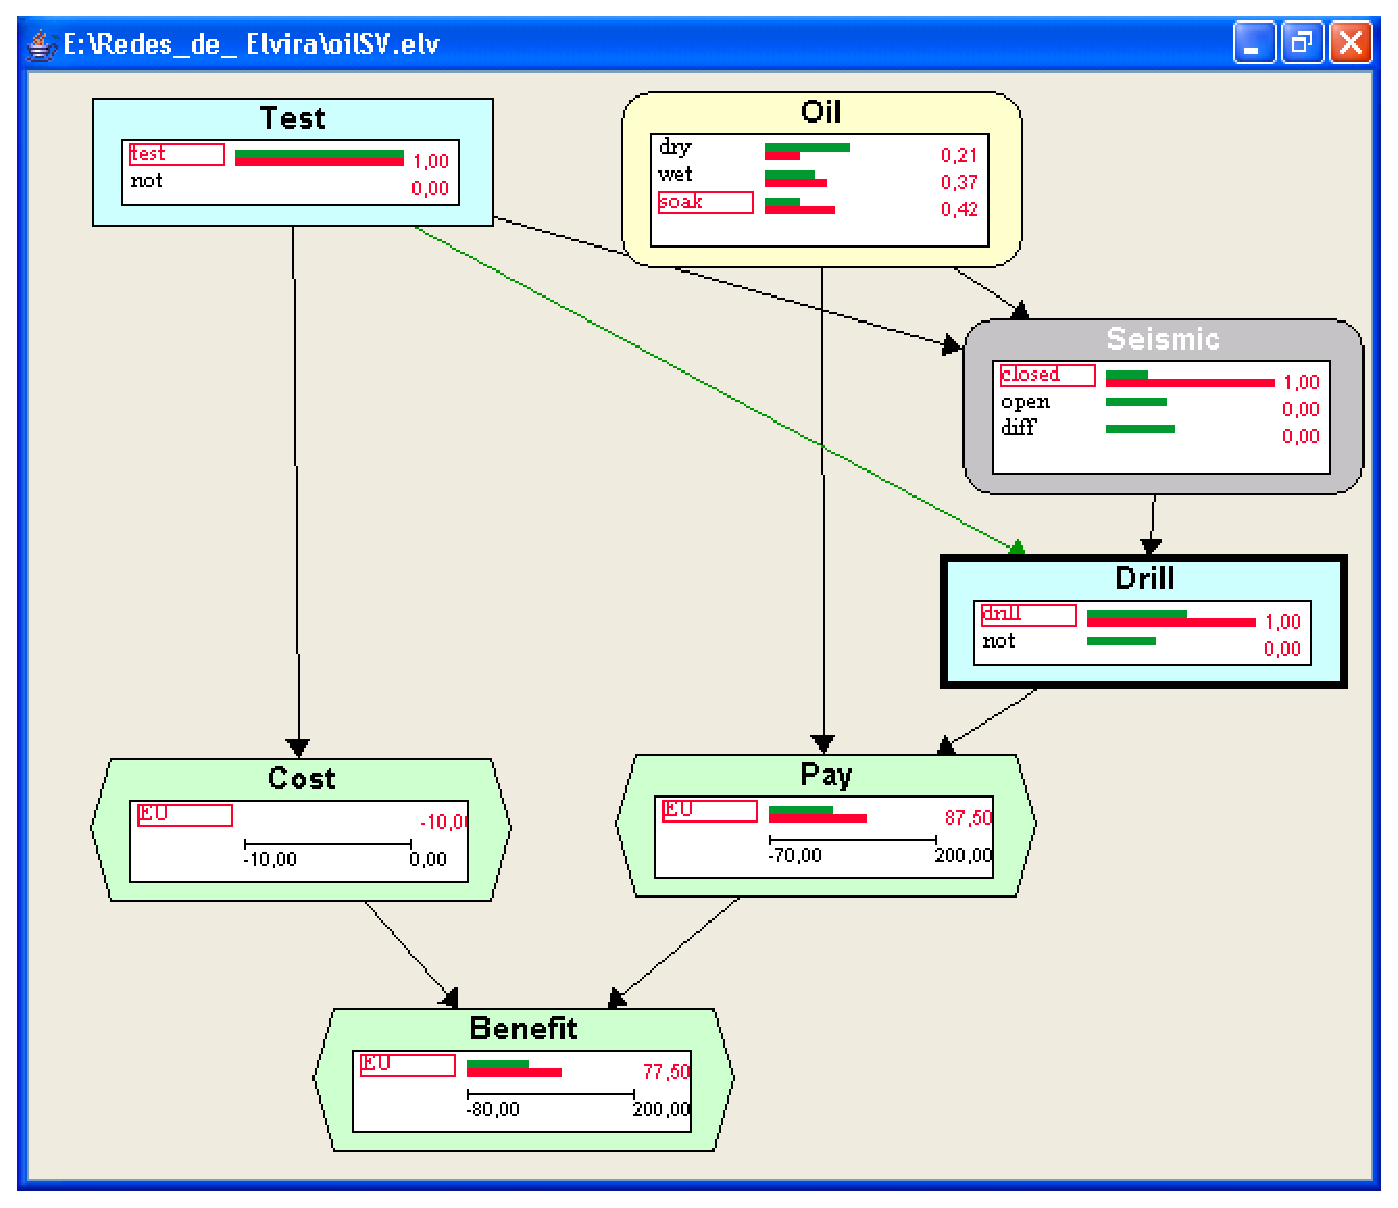
\includegraphics[scale=0.35]{./ID/fig/evaluatedCaseReactorIDSVGUI.eps} \vspace{-0.5cm}
\end{center}
\caption{Analysis of the optimal strategy}
\label{fig:evaluatedCaseReactorIDSVGUI}
\end{figure}
